


\documentclass[11pt,letterpaper]{article}

% Load some basic packages that are useful to have
% and that should be part of any LaTeX installation.
%
% be able to include figures
\usepackage{graphicx}
% get nice colors
\usepackage{xcolor}

% change default font to Palatino (looks nicer!)
\usepackage[latin1]{inputenc}
\usepackage{mathpazo}
\usepackage[T1]{fontenc}
% load some useful math symbols/fonts
\usepackage{latexsym,amsfonts,amsmath,amssymb}

% comfort package to easily set margins
\usepackage[top=1in, bottom=1in, left=1in, right=1in]{geometry}
\usepackage{hyperref}
\usepackage[all]{hypcap}
% control some spacings
%
% spacing after a paragraph\begin{figure}[bth]
\setlength{\parskip}{.15cm}
% indentation at the top of a new paragraph
\setlength{\parindent}{0.0cm}

\begin{document}

\begin{center}
\Large
Ay190 -- Worksheet 12\\
David Vartanyan\\
Date: \today
\end{center}

\section{}

Column 1 is the mass, Column 2 the radius, Column 3 is the temperature, Column 4 is the density, columny 5 is the infall velocity and Coulumn 6 is the electron fraction. Column 7 is the rotation velocity (0).

We differentiate temperature and density since the temperature plot has a small increase going outwards for a certain radii. We would not expect density bumps.

See Fig ~\ref{fig:1}.

\section{}
I create an equidistant grid and interpolate using inbuilt interpolate.splev.

\section{}
I follow the template from ws8. I run into trouble in 2 areas. First, I could not figure how to to extrapolate data to the origin of the star at radius 0. Thus, my boundary conditions were applied at radius $10^{7}$ cm. I do not know how inaccurate this will be. Second, the expression in equation 3 on ws12 does not reduce to expression 2 at outer radius. This is because expression three will evaluate density at the outer radius whereas two uses an integrated average to find msas.

You can see in Fig ~\ref{fig:2} that the endpoints do not agree, and near the 'origin' of $R=10^{7} $ cm we differ by about 3 orders. We plot error normalized to analytical solution to show convergence in Fig. ~\ref{fig:3}.

\begin{figure}[bth]
\centering
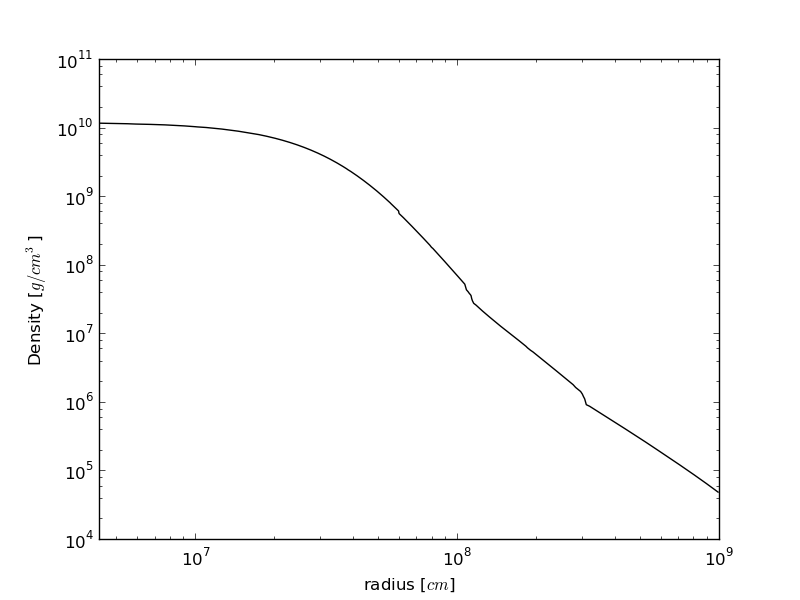
\includegraphics[width=0.7\textwidth]{ws12fig1.png}
\caption{Density vs Radius}
\label{fig:1}
\end{figure}


\begin{figure}[bth]
\centering
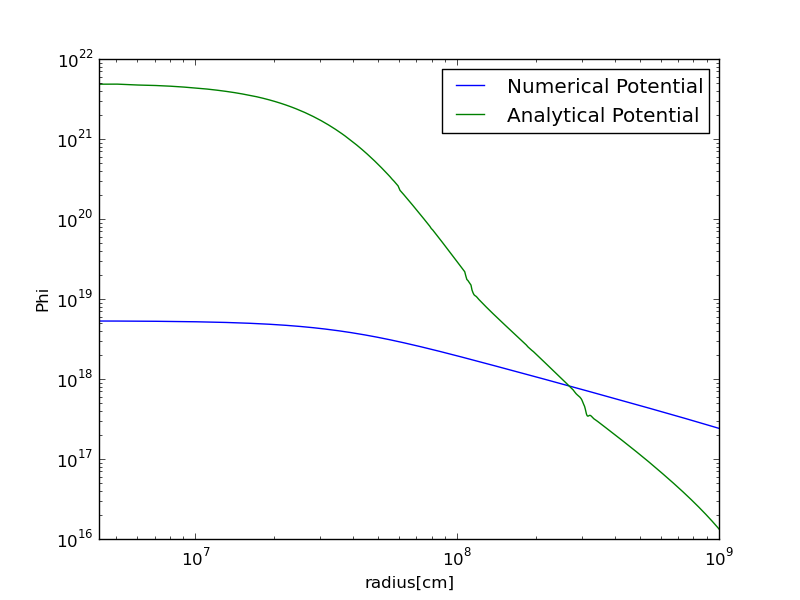
\includegraphics[width=0.7\textwidth]{ws12fig2.png}
\caption{Gravitational Potential vs Radius}
\label{fig:2}
\end{figure}


\begin{figure}[bth]
\centering
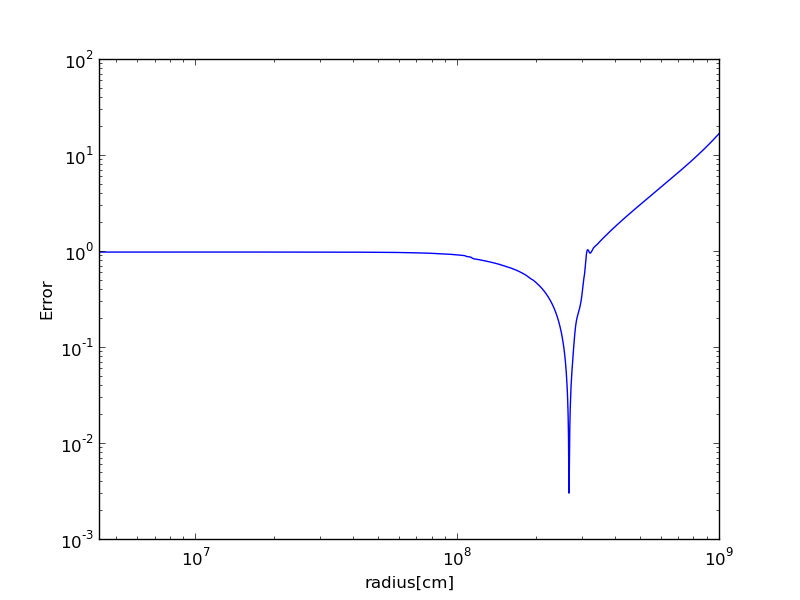
\includegraphics[width=0.7\textwidth]{ws12fig3.png}
\caption{Error vs Radius}
\label{fig:3}
\end{figure}

\end{document}
